%%
%% This is file `sample-acmsmall.tex',
%% generated with the docstrip utility.
%%
%% The original source files were:
%%
%% samples.dtx  (with options: `acmsmall')
%% 
%% IMPORTANT NOTICE:
%% 
%% For the copyright see the source file.
%% 
%% Any modified versions of this file must be renamed
%% with new filenames distinct from sample-acmsmall.tex.
%% 
%% For distribution of the original source see the terms
%% for copying and modification in the file samples.dtx.
%% 
%% This generated file may be distributed as long as the
%% original source files, as listed above, are part of the
%% same distribution. (The sources need not necessarily be
%% in the same archive or directory.)
%%
%% Commands for TeXCount
%TC:macro \cite [option:text,text]
%TC:macro \citep [option:text,text]
%TC:macro \citet [option:text,text]
%TC:envir table 0 1
%TC:envir table* 0 1
%TC:envir tabular [ignore] word
%TC:envir displaymath 0 word
%TC:envir math 0 word
%TC:envir comment 0 0
%%
%%
%% The first command in your LaTeX source must be the \documentclass command.
\documentclass[acmsmall,anonymous]{acmart}
%% NOTE that a single column version is required for 
%% submission and peer review. This can be done by changing
%% the \doucmentclass[...]{acmart} in this template to 
%% \documentclass[manuscript,screen]{acmart}
%% 
%% To ensure 100% compatibility, please check the white list of
%% approved LaTeX packages to be used with the Master Article Template at
%% https://www.acm.org/publications/taps/whitelist-of-latex-packages 
%% before creating your document. The white list page provides 
%% information on how to submit additional LaTeX packages for 
%% review and adoption.
%% Fonts used in the template cannot be substituted; margin 
%% adjustments are not allowed.
%%
%% \BibTeX command to typeset BibTeX logo in the docs
\AtBeginDocument{%
  \providecommand\BibTeX{{%
    \normalfont B\kern-0.5em{\scshape i\kern-0.25em b}\kern-0.8em\TeX}}}

%% Rights management information.  This information is sent to you
%% when you complete the rights form.  These commands have SAMPLE
%% values in them; it is your responsibility as an author to replace
%% the commands and values with those provided to you when you
%% complete the rights form.
\setcopyright{acmlicensed}
\copyrightyear{2018}
\acmYear{2018}
\acmDOI{XXXXXXX.XXXXXXX}


%%
%% These commands are for a JOURNAL article.
\acmJournal{JACM}
\acmVolume{37}
\acmNumber{4}
\acmArticle{111}
\acmMonth{8}

%%
%% Submission ID.
%% Use this when submitting an article to a sponsored event. You'll
%% receive a unique submission ID from the organizers
%% of the event, and this ID should be used as the parameter to this command.
%%\acmSubmissionID{123-A56-BU3}

%%
%% For managing citations, it is recommended to use bibliography
%% files in BibTeX format.
%%
%% You can then either use BibTeX with the ACM-Reference-Format style,
%% or BibLaTeX with the acmnumeric or acmauthoryear sytles, that include
%% support for advanced citation of software artefact from the
%% biblatex-software package, also separately available on CTAN.
%%
%% Look at the sample-*-biblatex.tex files for templates showcasing
%% the biblatex styles.
%%

%%
%% The majority of ACM publications use numbered citations and
%% references.  The command \citestyle{authoryear} switches to the
%% "author year" style.
%%
%% If you are preparing content for an event
%% sponsored by ACM SIGGRAPH, you must use the "author year" style of
%% citations and references.
%% Uncommenting
%% the next command will enable that style.
%%\citestyle{acmauthoryear}

%%
%% end of the preamble, start of the body of the document source.

\usepackage{mathtools}
\usepackage{amsmath}
\usepackage{ebproof}
\usepackage{xcolor}
\usepackage{listings}
\usepackage{mathpartir}

% !TEX root = ./main.tex

%%% Editing Convience Macros

\newif\ifdraft
\drafttrue
\newcommand{\TODO}[1]{\ifdraft{\textcolor{red}{\textbf{TODO}: {#1}}}\fi}
\newcommand{\mck}[1]{\ifdraft{\color{purple}[#1 --Matt]}\fi}
\newcommand{\hxf}[1]{\ifdraft{\color{blue}[#1 --Haoxiang]}\fi}

%%% Hazel language highlight

\lstdefinelanguage{hazel}{
  columns=fullflexible,
  keepspaces=true,
  basicstyle=\ttfamily\color{black},
  keywords={
    let, in, case, end, type,
    eval, pause, hide, debug
  },
  keywordstyle=\bfseries\color{black},
  commentstyle=\color{gray},
}

%%% Stepper/Filter Semantics

\DeclareMathSymbol{\Gamma}{\mathalpha}{operators}{0}
\DeclareMathSymbol{\Delta}{\mathalpha}{operators}{1}
\DeclareMathSymbol{\Theta}{\mathalpha}{operators}{2}
\DeclareMathSymbol{\Lambda}{\mathalpha}{operators}{3}
\DeclareMathSymbol{\Xi}{\mathalpha}{operators}{4}
\DeclareMathSymbol{\Pi}{\mathalpha}{operators}{5}
\DeclareMathSymbol{\Sigma}{\mathalpha}{operators}{6}
\DeclareMathSymbol{\Upsilon}{\mathalpha}{operators}{7}
\DeclareMathSymbol{\Phi}{\mathalpha}{operators}{8}
\DeclareMathSymbol{\Psi}{\mathalpha}{operators}{9}
\DeclareMathSymbol{\Omega}{\mathalpha}{operators}{10}


\DeclareMathOperator{\DefPat}{Pat}
\DeclareMathOperator{\DefExp}{Exp}
\DeclareMathOperator{\DefVal}{Val}
\DeclareMathOperator{\DefCtx}{Ctx}
\DeclareMathOperator{\DefAct}{Act}
\DeclareMathOperator{\DefGas}{Gas}
\DeclareMathOperator{\DefFilter}{Filter}
\DeclareMathOperator{\KeywordFilter}{filter}
\DeclareMathOperator{\KeywordResidue}{residue}
% \DeclareMathOperator{\Nat}{\mathsf{Nat}}

\newcommand{\Nat}[1]{\underline{#1}}
\newcommand{\Lam}[3]{\lambda #1 : #2 . #3}
\newcommand{\Filter}[4]{\KeywordFilter #1 ~\mathsf{do}~ #2 ~\mathsf{for}~ #3 ~\mathsf{in}~ #4}
\newcommand{\Residue}[4]{\mathsf{do}~ #1 ~\mathsf{for}~ #2 ~\mathsf{at}~ #3 ~\mathsf{in}~ #4}

\newcommand{\Value}[1]{#1~\mathsf{value}}
\newcommand{\FEStep}[2]{#1 \mapsto #2}
\newcommand{\FSubst}[3]{[#1/#2] #3}

\newcommand{\FCMark}{\circ}

\newcommand{\FASkip}{\mathsf{skip}}
\newcommand{\FAStep}{\mathsf{step}}
\newcommand{\FGOne}{\mathsf{one}}
\newcommand{\FGAll}{\mathsf{all}}

\DeclareMathOperator{\Strip}{strip}

\newcommand{\Decompose}[3]{#1 \Rightarrow #2 \{ #3 \}}
\newcommand{\Compose}[3]{#1 \Leftarrow #2 \{ #3 \}}

\newcommand{\Matches}[2]{#1 \mathrel{\mathop{\triangleright}} #2}
\newcommand{\FPatMatchesExpOp}{\mathrel{\mathop{\triangleright}}}
\newcommand{\FPatMatchesExp}[2]{#1 \FPatMatchesExpOp #2}
\newcommand{\FPatNotMatchesExpOp}{\mathrel{\mathop{\not\triangleright}}}
\newcommand{\FPatNotMatchesExp}[2]{#1 \FPatNotMatchesExpOp #2}

\newcommand{\FPatMatchesCtxOpL}{\mathrel{\mathop{\triangleright_\circ}}}
\newcommand{\FPatMatchesCtxOpR}{\mathrel{\mathop{\triangleleft_\circ}}}
\newcommand{\FPatMatchesCtx}[3]{#1 \FPatMatchesCtxOpL #2 \{ #3 \}}

\newcommand{\FInstruct}[3]{#1 \vdash #2 \rightsquigarrow #3}

\newcommand{\Analyze}[4]{#1 \vdash #2 \rightsquigarrow #3 \dashv #4}

\newcommand{\FTrans}[2]{#1 \rightarrow #2}

\newcommand{\FStep}[3]{#1 \vdash #2 \mapsto #3}

\newcommand{\FHasType}[3]{#1 \vdash #2 : #3}
\newcommand{\FInTypeContext}[3]{#1 : #2 \in #3}
\newcommand{\FTNat}{\mathbb{N}}

%%% Local Variables:
%%% mode: latex
%%% TeX-master: "main"
%%% End:


\newcommand{\evalsto}{\mathrel{\mathop{\Downarrow}}}
\newcommand{\matches}{\mathrel{\mathop{\blacktriangleright}}}
\newcommand{\fmatches}{\mathrel{\mathop{\triangleright}}}
\newcommand{\smatches}{\mathrel{\mathop{\sim}}}
\newcommand{\hooksto}{\mathrel{\mathop{\hookrightarrow}}}
\newcommand{\entails}{\mathrel{\mathop{\vdash}}}
\newcommand{\steps}{\mathrel{\mathop{\vartriangleright}}}
\newcommand{\skips}{\mathrel{\mathop{\blacktriangleright}}}
\newcommand{\final}{~\mathbf{final}}
\newcommand{\ival}{~\mathbf{value}}
\newcommand{\indet}{~\mathbf{indet}}
\newcommand{\istep}{~\mathbf{step}}
\newcommand{\iskip}{~\mathbf{skip}}
\newcommand{\class}[1]{\operatorname{#1}}
% \DeclareMathOperator{\Filter}{Filter}
\DeclareMathOperator{\askip}{\mathsf{skip}}
\DeclareMathOperator{\astep}{\mathsf{step}}
\DeclareMathOperator{\filter}{\mathsf{filter}}
\newcommand{\fin}{\mathrel{\mathop{\mathsf{in}}}}
\newcommand{\flet}{\operatorname{\mathsf{let}}}
\newcommand{\synth}{\mathrel{\mathop{\Rightarrow}}}
\newcommand{\analyze}{\mathrel{\mathop{\Leftarrow}}}
\newcommand{\ctype}[1]{\mathsf{#1}}
\newcommand{\inl}{\operatorname{\mathsf{injL}}}
\newcommand{\inr}{\operatorname{\mathsf{injR}}}
\newcommand{\prl}{\operatorname{\mathsf{prjL}}}
\newcommand{\prr}{\operatorname{\mathsf{prjR}}}
\newcommand{\MatchArrow}{\mathrel{\mathop{\blacktriangleright_{\rightarrow}}}}
\newcommand{\fif}{\operatorname{\mathsf{if}}}
\newcommand{\fthen}{\mathrel{\mathop{\mathsf{then}}}}
\newcommand{\felse}{\mathrel{\mathop{\mathsf{else}}}}
\newcommand{\fcase}{\operatorname{\mathsf{case}}}
\newcommand{\fcaseL}{\mathsf{L}}
\newcommand{\fcaseR}{\mathsf{R}}
\DeclareMathOperator{\instr}{\mathsf{instr}}

\begin{document}

%%
%% The "title" command has an optional parameter,
%% allowing the author to define a "short title" to be used in page headers.
\title{Stepper}

%%
%% The "author" command and its associated commands are used to define
%% the authors and their affiliations.
%% Of note is the shared affiliation of the first two authors, and the
%% "authornote" and "authornotemark" commands
%% used to denote shared contribution to the research.
\author{Ben Trovato}
\authornote{Both authors contributed equally to this research.}
\email{trovato@corporation.com}
\orcid{1234-5678-9012}
\author{G.K.M. Tobin}
\authornotemark[1]
\email{webmaster@marysville-ohio.com}
\affiliation{%
  \institution{Institute for Clarity in Documentation}
  \streetaddress{P.O. Box 1212}
  \city{Dublin}
  \state{Ohio}
  \country{USA}
  \postcode{43017-6221}
}

\author{Lars Th{\o}rv{\"a}ld}
\affiliation{%
  \institution{The Th{\o}rv{\"a}ld Group}
  \streetaddress{1 Th{\o}rv{\"a}ld Circle}
  \city{Hekla}
  \country{Iceland}}
\email{larst@affiliation.org}

\author{Valerie B\'eranger}
\affiliation{%
  \institution{Inria Paris-Rocquencourt}
  \city{Rocquencourt}
  \country{France}
}

\author{Aparna Patel}
\affiliation{%
 \institution{Rajiv Gandhi University}
 \streetaddress{Rono-Hills}
 \city{Doimukh}
 \state{Arunachal Pradesh}
 \country{India}}

\author{Huifen Chan}
\affiliation{%
  \institution{Tsinghua University}
  \streetaddress{30 Shuangqing Rd}
  \city{Haidian Qu}
  \state{Beijing Shi}
  \country{China}}

\author{Charles Palmer}
\affiliation{%
  \institution{Palmer Research Laboratories}
  \streetaddress{8600 Datapoint Drive}
  \city{San Antonio}
  \state{Texas}
  \country{USA}
  \postcode{78229}}
\email{cpalmer@prl.com}

\author{John Smith}
\affiliation{%
  \institution{The Th{\o}rv{\"a}ld Group}
  \streetaddress{1 Th{\o}rv{\"a}ld Circle}
  \city{Hekla}
  \country{Iceland}}
\email{jsmith@affiliation.org}

\author{Julius P. Kumquat}
\affiliation{%
  \institution{The Kumquat Consortium}
  \city{New York}
  \country{USA}}
\email{jpkumquat@consortium.net}

%%
%% By default, the full list of authors will be used in the page
%% headers. Often, this list is too long, and will overlap
%% other information printed in the page headers. This command allows
%% the author to define a more concise list
%% of authors' names for this purpose.
\renewcommand{\shortauthors}{Trovato and Tobin, et al.}

%%
%% The abstract is a short summary of the work to be presented in the
%% article.
\begin{abstract}
  A clear and well-documented \LaTeX\ document is presented as an
  article formatted for publication by ACM in a conference proceedings
  or journal publication. Based on the ``acmart'' document class, this
  article presents and explains many of the common variations, as well
  as many of the formatting elements an author may use in the
  preparation of the documentation of their work.
\end{abstract}

%%
%% The code below is generated by the tool at http://dl.acm.org/ccs.cfm.
%% Please copy and paste the code instead of the example below.
%%
\begin{CCSXML}
<ccs2012>
 <concept>
  <concept_id>00000000.0000000.0000000</concept_id>
  <concept_desc>Do Not Use This Code, Generate the Correct Terms for Your Paper</concept_desc>
  <concept_significance>500</concept_significance>
 </concept>
 <concept>
  <concept_id>00000000.00000000.00000000</concept_id>
  <concept_desc>Do Not Use This Code, Generate the Correct Terms for Your Paper</concept_desc>
  <concept_significance>300</concept_significance>
 </concept>
 <concept>
  <concept_id>00000000.00000000.00000000</concept_id>
  <concept_desc>Do Not Use This Code, Generate the Correct Terms for Your Paper</concept_desc>
  <concept_significance>100</concept_significance>
 </concept>
 <concept>
  <concept_id>00000000.00000000.00000000</concept_id>
  <concept_desc>Do Not Use This Code, Generate the Correct Terms for Your Paper</concept_desc>
  <concept_significance>100</concept_significance>
 </concept>
</ccs2012>
\end{CCSXML}

\ccsdesc[500]{Do Not Use This Code~Generate the Correct Terms for Your Paper}
\ccsdesc[300]{Do Not Use This Code~Generate the Correct Terms for Your Paper}
\ccsdesc{Do Not Use This Code~Generate the Correct Terms for Your Paper}
\ccsdesc[100]{Do Not Use This Code~Generate the Correct Terms for Your Paper}

%%
%% Keywords. The author(s) should pick words that accurately describe
%% the work being presented. Separate the keywords with commas.
\keywords{Do, Not, Us, This, Code, Put, the, Correct, Terms, for,
  Your, Paper}

\received{20 February 2007}
\received[revised]{12 March 2009}
\received[accepted]{5 June 2009}

%%
%% This command processes the author and affiliation and title
%% information and builds the first part of the formatted document.
\maketitle

\section{Introduction}

Debugger has been one of the most important tools that students and programmer
use to learn the behavior of their programs. Well-established debuggers such as
GDB, LLDB, and Visual Studio Debugger have been widely used in industry and
academia. These debuggers provide rich set of tools for user to inspect and even
change various aspects of a running program, such as memory, variables,
and call stacks. However, they also suffers from several limitations.

\begin{enumerate}
  \item They are tailored for imperative languages like C or C++. They are not
    well-suited for functional languages, where memory is usually managed by
    GC and never directly manipulated by the programmer.
  \item Many of them support stepping in and stepping over instructions. However,
    these two instructions can be tedious to use when the program is large and
    complex. The user has to step through many instructions that are not relevant
    to the current task.
  \item They are not well-suited for teaching. They are designed for professional
    programmers who are already familiar with the language and the program they
    are debugging. They are not well-suited for beginners who are learning the
    language and the program.
\end{enumerate}

Therefore, we want to develop a new kind of debugger that tailored for
functional languages and is well-suited for teaching in Hazel. Hazel is a pure
functional language that supports working with incomplete programs. It is used
in a upper-level programming languages course where we are teaching
substitution-based equational semantics -- we want the steps to show up as
justified proof steps, to mirror what we have previously done in lectures and
written assignments.

\TODO{(example here of a simple equational stepping proof)}

One of the main challenges in using such a debugger in lecturing is that it is
often tedious to step through a program. Students has to witness many boring
instructions that are not relevant to the current task, or that they already
well understand. Those instructions will litter the proof and obscure the key
idea. Our approach is to develop a scoped filter system that allows us to write patterns
that will be skipped or paused. For example,

\TODO{(more sophisticated example where you show side-by-side the unfiltered and
filtered version of the same stepping sequence) fib, foldright, map}

Our scoped filter system allows the user to specify sub-expressions whose full
evaluation they are not interested in, sub-expressions whose full evaluation
they are interested in, specific steps they are not interested in, and specific
steps they are interested in.

\TODO{want to be able to step programs with holes, including error holes:
abstract foldright vs foldleft}

% Prior work summary: what have people tried to do to handle this challenge in the past? why is that not quite enough

We have made the following contributes in the paper:
\begin{itemize}
  \item We have developed the hazel stepper and a companion scoped filter system
    that allows the user to specify sub-expressions whose full evaluation they
    are not interested in, sub-expressions whose full evaluation they are
    interested in, specific steps they are not interested in, and specific steps
    they are interested in.
  \item We have deployed the hazel stepper and the scoped filter system in
    lecture and to students. We have conducted qualitative and quantitative
    evaluation of the system.
  \item We have formalized the filter semantics and proved the meta-theory
    theorems of the hazel filter system so that we can be confident that the
    filter system have desired properties.
\end{itemize}

% - developed the hazel stepper and filter system, implemented it, deployed it in lecture (qualitative evaluation), deployed it to students (qualitative + quantitative evaluation), formalized the filter semantics, metatheory


\section{Hazel Stepper by Example}

In this section, we introduce the Hazel stepper filter.

We recognized some key capabilities that traditional debuggers have and will be
also helpful to a debugger for functional programming languages.
\begin{enumerate}
  \item Evaluation can be paused at some point and resumed later. The user
    should be able specify where/when the evaluation should be paused. This is
    usually implemented as the breakpoint mechanism in a traditional debugger.
  \item Paused evaluation can be stepped through. traditionally, debuggers will
    provide user with three buttons to ``step through'', ``step over'' and
    ``step out''.
\end{enumerate}

Moreover, we want some extra capabilities that are specific to functional
programming languages and a classroom settings, especially Hazel, to be a
useful tool for teaching and learning functional programming.
\begin{enumerate}
  \item It can skip the stepping process of some \emph{kind} of expression.
  \item It controls the evaluation of the program in a granularity of
  expression, instead of a granularity of line or instruction.ß
\end{enumerate}

To serve as a good tool for understanding the behavior of a program, the stepper
filter should have consistent behavior with the semantics of the language. Hazel
internally uses a environment-based big-step evaluator to evaluate the program,
but it has a consistent behavior with the substitution-based one. Therefore,
the stepper filter shall not exhibit different behavior when building upon a
environment-based evaluator or a substitution-based evaluator.

The evaluation order of Hazel is not specified. Therefore, an expression that is
not value might have multiple possible choice 

\subsection{Matching}


Terms that has the same structural form after substituting all bounded variables
are considered \emph{matched}.

\begin{verbatim}
let x = 3 in
eval x + 3 in
x + 3
\end{verbatim}
shall has the same behavior as the program
\begin{verbatim}
let x = 3 in
eval 3 + 3 in
3 + 3
\end{verbatim}

\begin{verbatim}
eval $e in
let g = fun x -> x + x in
pause g($v) in # or pause (fun x -> x + x)($v) in
(fun x -> x + x)(3)
== (fun x -> x + x)(3) # or g(3) #
\end{verbatim}

\begin{figure}[h]
  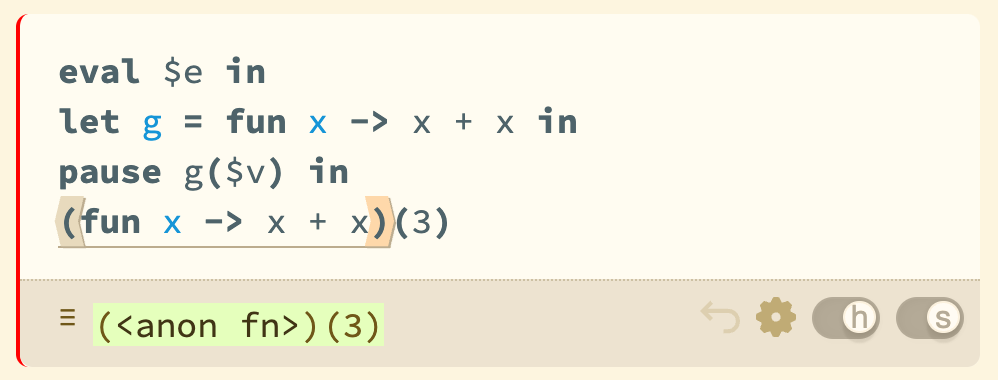
\includegraphics[width=0.4\textwidth]{images/match-mod-subst.png}
\end{figure}

As in a substitution-based evaluator, the substitution is applied to the
the body of a function:
\begin{verbatim}
eval $e in
let y = fun x -> x in
let h = fun x -> (fun y -> y) in
pause (fun x -> y)($v) in
h(3)
== h(3) # or (fun x -> (fun x -> x))(3) #
\end{verbatim}

\begin{figure}[h]
  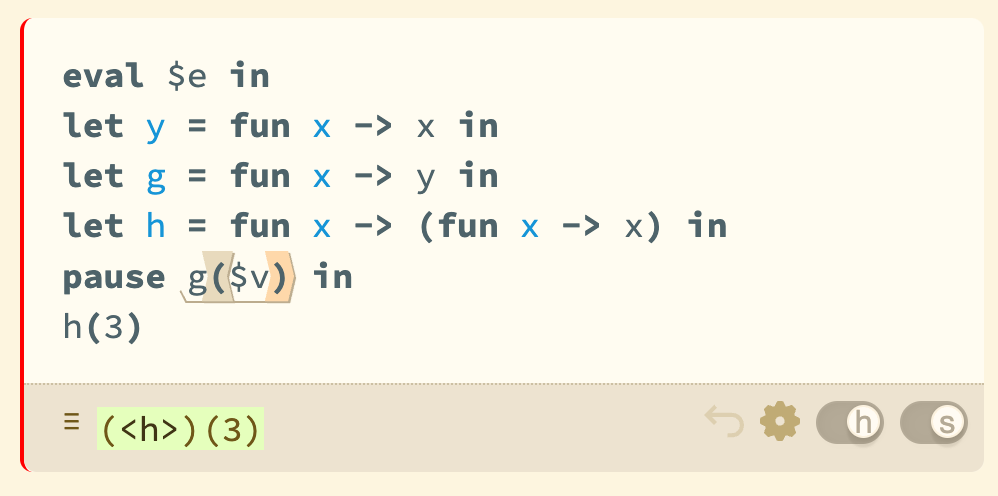
\includegraphics[width=0.4\textwidth]{images/match-recursive.png}
\end{figure}

A immediate corollary of this is that the stepper filter shows that
the filter cannot be applied to a variable, since the substitution is always
performed ahead of the matching process, and for the filter it shall not be
able to match against a variable.

\begin{verbatim}
eval $e in
let x = 3 in
pause x in
x + x
== 6
\end{verbatim}

\TODO{Discuss: whether or not to use alpha-equivalence here.}

\subsection{Four filters: Hide, Eval, Pause and Debug}

\TODO{Discuss: mention skip all, skip one, pause all and all one?}

Typical use case for the four basic filters.

\paragraph{eval} We want to use the \verb|eval| to \emph{evaluate} all sub-expressions that matches the pattern.
\begin{verbatim}
eval 1 + 2 in
1 + 2
== 3
\end{verbatim}

We want the \verb|hide| filters to hide away one step.
\begin{verbatim}
hide let   =   in   in
let x = 3 in
let y = 4 in
x + y
== 3 + 4
== 7
\end{verbatim}
while using \verb|eval| it will behave like this:
\begin{verbatim}
eval let   =   in   in
let x = 3 in
let y = 4 in
x + y
== 7
\end{verbatim}

\paragraph{hide} The \verb|hide| filter will be \emph{used up} when its body
expression is actually being evaluated.

During evaluation, we want to be able to examine every instruction
transitioning steps.

\begin{verbatim}
eval 1 + 2 + 3 + 4 in
pause 3 + 3 in
1 + 2 + 3 + 4
== 3 + 3 + 4
== 10
\end{verbatim}

This would be especially useful when unfolding a higher level
expression to its individual terms, for example I want to know how
many terms of \verb|fib(1)| I need to call to evaluate the whole
\verb|fib(5)|.

On the other hand, we want to went through all the evaluation process of a
sub-expression, for example when debugging the implementation of a function
\begin{verbatim}
let (is_even: Int -> Bool, is_odd: Int -> Bool) = ... in
debug is_odd($v) in
is_even(5)
\end{verbatim}

The difference between \verb|pause| and \verb|debug| is subtle. For
example, considering the following two piece of code:
\begin{verbatim}
eval $e in
pause (1 + 2) + (3 + 4) + (5 + 6) in
eval 3 + 7 + (5 + 6) in
(1 + 2) + (3 + 4) + (5 + 6)
== (1 + 2) + (3 + 4) + (5 + 6)
== 21
\end{verbatim}
and
\begin{verbatim}
eval $e in
debug (1 + 2) + (3 + 4) + (5 + 6) in
eval 3 + 7 + (5 + 6) in
(1 + 2) + (3 + 4) + (5 + 6)
== (1 + 2) + (3 + 4) + (5 + 6)
== 3 + (3 + 4) + (5 + 6)
== 21
\end{verbatim}
The first one will immediately evaluate to final value is because it is a \verb|pause| statement, which will be only effective once.

Filters can't be applied on values. A more significant corollary of this is they cannot be applied on variables as well.
\begin{verbatim}
eval $e in
pause x in
pause y in
let x = 3 in
let y = 4 in
x + y
== 7
\end{verbatim}

\subsection{Interaction between filter statements}

\TODO{Q: Do we need formalise these properties?}

We want nested filter statements to behave correctly, i.e.
\begin{enumerate}
\item For every pattern \verb|p|, \verb|pause p| cancels the effects
  of \verb|eval p| and \verb|hide p|, vice versa.
\item Inner filter statements take precedences.
\end{enumerate}

\begin{verbatim}
pause 1 + 2 + 3 + 4 in
eval 1 + 2 + 3 + 4 in
1 + 2 + 3 + 4
== 10
\end{verbatim}

\begin{verbatim}
pause $e in
eval 1 + 2 + 3 + 4 in
pause 1 + 2 + 3 + 4 in
1 + 2 + 3 + 4
== 1 + 2 + 3 + 4
\end{verbatim}

\begin{verbatim}
pause $e in
hide (let   =   in  ) in
pause (let   =   in  ) in
let x = 3 in
x + 4
== let x = 3 in x + 4
\end{verbatim}

The nesting properties should works across bindings.

\begin{verbatim}
eval $e in
let x = 1 in
pause 3 + 3 in
let y = 2 in
eval 3 + 3 in
x + y + 3 + 4
== 10
\end{verbatim}

\begin{verbatim}
let add = fun x, y -> pause $e in x + y in
eval $e in
add(3, 4)
== [3 + 4]
\end{verbatim}

We want the filter to recover to \emph{older} state when it finish
evaluating matched sub-expression.

\begin{verbatim}
pause $e in
eval 1 + 2 + 3 + 4 in
pause 3 + 3 in
1 + 2 + 3 + 4
== 3 + 3 + 4
== 10
\end{verbatim}

After evaluating \verb|3 + 3|, the stepper falls back to eval mode
since eval filter matches \verb|1 + 2 + 3 + 4|, so it directly
evaluates to \verb|10|.

We also want a \verb|eval| filter to automatically evaluate all sub-expression
until it cannot proceed.

\subsection{Handling inconsistency between DHExp and UExp}

\TODO{Discuss: Move to implementation.tex?}

There are inconsistencies between the surface expression and expression for
evaluation in Hazel. For example, fix-points are inserted in the expression
during elaboration. We want the filters to work with fix-points, with-out user
acknowledging that they actually needs a fix-point to implement the recursion.

\begin{verbatim}
let map : ([Int], Int -> Int) -> [Int] = fun xs, f ->
  case xs
  | [] => []
  | hd :: tl => f(hd)::map(tl, f)
  end
in
let square = fun x -> x * x in
pause map($v) in
map([1, 2, 3], square)
== 1::map([2, 3], f)
== 1::4::map([3], f)
\end{verbatim}

In the example above, we don't want to use to click twice to do unroll and apply, instead we want to merge these two transition
in one step.

\subsection{Good but unrealistic for now}

\TODO{Discuss: Is it better remove in total?}

There are also something that we think would be intuitive and useful but not possible with current implementation

\begin{verbatim}
let fib : Int -> Int =
  fun n ->
    if n <= 1 then
      n
    else
      fib(n - 1) + fib(n - 2)
in
pause fib($v) + fib($v) in
fib(5)
== 3
\end{verbatim}

Intuitively we shall see a evaluation trace like this:
\begin{verbatim}
...
== fib(4) + fib(3)
== fib(3) + fib(2) + fib(3)
== fib(3) + fib(2) + fib(2) + fib(1)
== ...
\end{verbatim}

This is no possible since this require us to traverse all possible
evaluation sequence given a program, which would be super powerful,
but at the same time super slow.

%%% Local Variables:
%%% mode: latex
%%% TeX-master: "main"
%%% End:


(think about examples that touch on all the edge cases of the system) 

(show substitutions explicitly)

\section{Filter Semantic Rules}

\subsection{Definitions}

\fbox{\(\DefAct a\)} Action \(a\) of a filter
\[
  \DefAct a \Coloneqq \FASkip \mid \FAStep
\]

\fbox{\(\DefGas g\)} Gas \(g\) of a filter.
\[
  \DefGas g \Coloneqq \FGOne \mid \FGAll
\]

\fbox{\(\DefExp d\)} Expression \(d\).
\[
  \DefExp d \Coloneqq x \mid d(d) \mid \Lam{x}{d} \mid d + d \mid \Nat{n} \mid \Filter{p}{a}{g}{d} \mid \Residue{a}{g}{l}{d}
\]

% \fbox{\(\DefVal d\)} Value \(v\).
% \[
%   \DefVal v \Coloneqq \Lam{x}{d} \mid \Nat{n}
% \]

% \mck{I added a value thing here but we should probably actually define it as a judgement instead.}

\fbox{\(\DefCtx \mathcal{E}\)} Context \(\mathcal{E}\).
\[
  \DefCtx \mathcal{E}
  = \FCMark
  \mid \mathcal{E}(d)
  \mid d(\mathcal{E})
  \mid \mathcal{E} + d
  \mid d + \mathcal{E}
  \mid \Filter{p}{a}{g}{l}{\mathcal{E}}
  \mid \Residue{a}{g}{l}{\mathcal{E}}
\]

% \mck{Maybe replace $\Residue{a}{g}{l}{\mathcal{E}}$ with $\Residue{a}{\FGAll}{l}{\mathcal{E}}$ because only $\FGAll$ is possible?}

\fbox{\(\DefPat p\)} Pattern \(p\).
\[
  \DefPat p \Coloneqq \$e \mid \$v \mid x \mid p(p) \mid \Lam{x}{d} \mid p + p \mid \Nat{n}
\]

% \mck{The $\lambda \$x. $ form actually isn't necessary because we use alpha-equivalence later.}

\fbox{\(\DefFilter f\)} Filter \(f\).
\[
  \DefFilter f = (p, a, g)
\]

\subsection{Dynamics}

\fbox{\(\Value e\)} Expression \(e\) is a value.
\begin{mathpar}
  \inferrule[V-Lam]{
  }{
    \Value{\Lam{x}{d}}
  } \qquad
  \inferrule[V-Nat]{
  }{
    \Value{\Nat{n}}
  }
\end{mathpar}

\fbox{\([x / v] e = e'\)} \(e'\) can be obtained by substitution of \(x\) for
\(v\) in \(e\).
\[
  \begin{aligned}
    [x / v] x &= v \\
    [x / v] y &= y && \text{if } x \neq y \\
    [x / v] (e_1(e_2)) &= ([x / v] e_1)([x / v] e_2) \\
    [x / v] \Lam{y}{\tau}{e} &= \Lam{y}{\tau}{[x / v] e} && \text{if } x \neq y \\
    [x / v] \Lam{y}{\tau}{e} &= \Lam{y}{\tau}{e} && \text{if } x = y \\
  \end{aligned}
\]
\hxf{Do we really need a judgement for substitution?}
% \begin{mathpar}
%   \inferrule[S-Var-Eq]{
%   }{
%     [x / v] x = v
%   } \qquad
%   \inferrule[S-Var-Neq]{
%     x \neq y
%   }{
%     [x / v] y = y
%   } \\
%   \inferrule[S-Ap]{
%   }{
%     [x / v] (e_1(e_2)) = ([x / v] e_1)([x / v] e_2)
%   } \\
%   \inferrule[S-Lam-Eq]{
%   }{
%     [x / v] \Lam{x}{\tau}{e} = \Lam{x}{\tau}{e}
%   } \qquad
%   \inferrule[S-Lam-Neq]{
%     x \neq y
%   }{
%     [x / v] \Lam{y}{\tau}{e} = \Lam{y}{\tau}{[x / v] e}
%   } \\
% \end{mathpar}

\mck{It might be clearer if we write out a separate recompose judgement too. I think decompose and recompose behave differently especially with regard to do statements}

\fbox{\(\Decompose{d}{\mathcal{E}}{d'}\)} Expression \(d\) can be obtained by putting expression \(d'\) into the mark of \(\mathcal{E}\).
\begin{mathpar}
  \inferrule[D-Var]{
  }{
    \Decompose{x}{\FCMark}{x}
  } \\
  \inferrule[D-Residue-I]{
    \Decompose{e}{\mathcal{E}}{e'}
  }{
    \Decompose{\Residue{a}{g}{l}{e}}{\mathcal{E}}{\Residue{a}{g}{l}{e'}}
  } \\
  \inferrule[D-Residue-E]{
    \Value{v}
  }{
    \Decompose{\Residue{a}{g}{l}{v}}{\circ}{\Residue{a}{g}{l}{v}}
  } \\
  \inferrule[D-Filter-I]{
    \Decompose{e}{\mathcal{E}}{e'}
  }{
    \Decompose{\Filter{p}{a}{g}{e}}{\mathcal{E}}{\Filter{p}{a}{g}{e'}}
  } \\
  \inferrule[D-Filter-E]{
    \Value{v}
  }{
    \Decompose{\Residue{p}{a}{g}{v}}{\circ}{\Residue{p}{a}{g}{v}}
  } \\
  \inferrule[D-Ap-L]{
    \Decompose{d_1}{\mathcal{E}_1}{d_1'}
  }{
    \Decompose{d_1(d_2)}{\mathcal{E}_1(d_2)}{d_1'}
  } \qquad
  \inferrule[D-Ap-R]{
    \Value{d_1} \\
    \Decompose{d_2}{\mathcal{E}_2}{d_2'}
  }{
    \Decompose{d_1(d_2)}{d_1(\mathcal{E}_2)}{d_2'}
  } \qquad
  \inferrule[D-Ap-E]{
    \Value{e_1} \\
    \Value{e_2}
  }{
    \Decompose{e_1(e_2)}{\circ}{e_1(e_2)}
  } \\
  \inferrule[D-Add-L]{
    \Decompose{d_1}{\mathcal{E}_1}{d_1'}
  }{
    \Decompose{d_1 + d_2}{\mathcal{E}_1 + d_2}{d_1'}
  } \qquad
  \inferrule[D-Add-R]{
    \Value{d_1} \\
    \Decompose{d_2}{\mathcal{E}_2}{d_2'}
  }{
    \Decompose{d_1 + d_2}{d_1 + \mathcal{E}_2}{d_2'}
  } \qquad
  \inferrule[D-Add-E]{
    \Value{e_1} \\
    \Value{e_2}
  }{
    \Decompose{e_1 + e_2}{\circ}{e_1 + e_2}
  }
\end{mathpar}
\mck{D-Filter-E rule does not have any filters in it}

\mck{The last four rules seem to specify an evaluation order - is this desired behaviour? I thought we were going to mention the nondeterminism somewhere in the text}

\mck{Todo: remove the unused `output' g from the above - I think we can also remove the `input` g too?}

\fbox{\(\Compose{d}{\mathcal{E}}{d'}\)} Expression \(d\) can be obtained by putting expression \(d'\) into the mark of \(\mathcal{E}\).
\begin{mathpar}
  \inferrule[C-Top]{
    \ 
  }{
    \Compose{e}{\circ}{e}
  } \qquad
  \inferrule[C-Ap-L]{
    \Compose{e_l}{\mathcal{E}}{e}
  }{
    \Compose{e_l(e_r)}{\mathcal{E}(e_r)}{e}
  } \qquad
  \inferrule[C-Ap-R]{
    \Compose{e_r}{\mathcal{E}}{e}
  }{
    \Compose{e_l(e_r)}{e_l(\mathcal{E})}{e}
  } \\
  \inferrule[C-Add-L]{
    \Compose{e_l}{\mathcal{E}}{e}
  }{
    \Compose{e_l + e_r}{\mathcal{E} + e_r}{e}
  } \qquad
  \inferrule[C-Add-R]{
    \Compose{e_r}{\mathcal{E}}{e}
  }{
    \Compose{e_l + e_r}{e_l + \mathcal{E}}{e}
  } \\
  \inferrule[C-Filter]{
    \Compose{e'}{\mathcal{E}}{e}
  }{
    \Compose{\Filter{p}{a}{g}{e'}}{\Filter{p}{a}{g}{\mathcal{E}}}{e}
  } \\
  \inferrule[C-Residue]{
    \Compose{e'}{\mathcal{E}}{e}
  }{
    \Compose{\Residue{a}{g}{l}{e'}}{\Residue{a}{g}{l}{\mathcal{E}}}{e}
  }
\end{mathpar}

\fbox{\(e_1 \equiv_\alpha e_2\)} \(e_1\) is alpha-equivalent to \(e_2\).
\begin{mathpar}
  \inferrule[\(\alpha\)-Var]{
  }{
    x \equiv_\alpha x
  } \qquad
  \inferrule[\(\alpha\)-Lam]{
    e_1 \equiv_\alpha [x_2/x_1](e_2)
  }{
    \Lam{x_1}{\tau_1}{e_1} \equiv_\alpha \Lam{x_2}{\tau_2}{e_2}
  } \\
  \inferrule[\(\alpha\)-Ap]{
    e_1 \equiv_\alpha e_3 \\
    e_2 \equiv_\alpha e_4
  }{
    e_1(e_2) \equiv_\alpha e_3(e_4)
  } \qquad
  \inferrule[\(\alpha\)-Add]{
    e_1 \equiv_\alpha e_3 \\
    e_2 \equiv_\alpha e_4
  }{
    e_1 + e_2 \equiv_\alpha e_3 + e_4
  } \\
  \inferrule[\(\alpha\)-Filter]{
    e_1 \equiv_\alpha e_2
  }{
    \Filter{p}{a}{g}{e_1} \equiv_\alpha \Filter{p}{a}{g}{e_2}
  } \\
  \inferrule[\(\alpha\)-Residue]{
    e_1 \equiv_\alpha e_2
  }{
    \Residue{a}{g}{l}{e_1} \equiv_\alpha \Residue{a}{g}{l}{e_2}
  }
\end{mathpar}

\fbox{\(\Strip{e} = {e'}\)} Strip expression \(e\) to get expression \(e'\).
\[
  \begin{aligned}
    \Strip{x} &= x \\
    \Strip{\Lam{x}{\tau}{e}} &= \Lam{x}{\tau}{\Strip{e}} \\
    \Strip{e_1(e_2)} &= (\Strip{e_1})(\Strip{e_2}) \\
    \Strip{\Nat{n}} &= \Strip{\Nat{b}} \\
    \Strip{e_1 + e_2} &= (\Strip{e_1}) + (\Strip{e_2}) \\
    \Strip{\Filter{p}{a}{g}{e}} &= \Strip{e} \\
    \Strip{\Residue{a}{g}{l}{e}} &= \Strip{e}
  \end{aligned}
\]

\fbox{\(\Matches{p}{d}\)} means that pattern \(p\) matches expression \(d\).
\begin{mathpar}
  \inferrule[M-All]{\ }{
    \Matches{\$e}{d}
  } \qquad
  \inferrule[M-Val]{\Value{v}}{
    \Matches{\$v}{v}
  } \\
  \inferrule[M-Nat]{
    m = n
  }{
    \Matches{\Nat{m}}{\Nat{n}}
  }\qquad
  \inferrule[M-Lam]{
    \Lam{x}{\tau_p}{e_p} \equiv_{\alpha} \Lam{y}{\tau_e}{e_e}
  }{
    \Matches{\Lam{x}{\tau_p}{e_p}}{\Lam{y}{\tau_e}{e_e}}
  } \\ 
  \inferrule[M-Ap]{
    \Matches{p_1}{d_1} \\
    \Matches{p_2}{d_2}
  }{
    \Matches{p_1(p_2)}{d_1(d_2)}
  } \qquad
  \inferrule[M-Add]{
    \Matches{p_1}{d_1} \\
    \Matches{p_2}{d_2}
  }{
    \Matches{p_1 + p_2}{d_1 + d_2}
  } \qquad
\end{mathpar}

\mck{M-Lam doesn't allow \$e inside function bodies - is this intentional?}

\fbox{\(\FInstruct{(p, a, g, l)}{d}{d'}\)} \(d\) is dynamically instructed to \(d'\).
\begin{mathpar}
  \inferrule[FI-V]{
    \Value{d}
  }{
    \FInstruct{(p, a, g, l)}{d}{d}
  } \\
  \inferrule[FI-Var-Y]{
    \FPatMatchesExp{p}{x}
  }{
    \FInstruct{(p, a, g, l)}{x}{\Residue{a}{g}{l}{x}}
  } \qquad
  \inferrule[FI-Var-N]{
    \FPatNotMatchesExp{p}{x}
  }{
    \FInstruct{(p, a, g, l)}{x}{x}
  } \\
  \inferrule[FI-I]{
    \FInstruct{(p_0, a_0, g_0, l_0)}{d_0}{d} \\
    \FInstruct{(p, a, g, l_0 + 1)}{d}{d'}
  }{
    \FInstruct{(p_0, a_0, g_0, l_0)}{\Filter{p}{a}{g}{d_0}}{\Filter{p}{a}{g}{d'}}
  } \\
  \inferrule[FI-T]{
    \FInstruct{(p_0, a_0, g_0, l_0)}{d_0}{d} \\
  }{
    \FInstruct{(p_0, a_0, g_0, l_0)}{\Residue{a}{g}{l}{d_0}}{\Residue{a}{g}{l}{d'}}
  } \\
  \inferrule[FI-Ap-Y]{
    \FInstruct{(p, a, g, l)}{d_1}{d_1'} \\
    \FInstruct{(p, a, g, l)}{d_2}{d_2'} \\
    \FPatMatchesExp{p}{d_1(d_2)}
  }{
    \FInstruct{(p, a, g, l)}{d_1(d_2)}{\Residue{a}{g}{l}{d_1'(d_2')}}
  } \\
  \inferrule[FI-Ap-N]{
    \FInstruct{(p, a, g, l)}{d_1}{d_1'} \\
    \FInstruct{(p, a, g, l)}{d_2}{d_2'} \\
    \FPatNotMatchesExp{p}{d_1(d_2)}
  }{
    \FInstruct{(p, a, g, l)}{d_1(d_2)}{d_1'(d_2')}
  } \\
  \inferrule[FI-Add-Y]{
    \FInstruct{(p, a, g, l)}{d_1}{d_1'} \\
    \FInstruct{(p, a, g, l)}{d_2}{d_2'} \\
    \FPatMatchesExp{p}{d_1 + d_2}
  }{
    \FInstruct{(p, a, g, l)}{d_1(d_2)}{\Residue{a}{g}{l}{d_1' + d_2'}}
  } \\
  \inferrule[FI-Add-N]{
    \FInstruct{(p, a, g, l)}{d_1}{d_1'} \\
    \FInstruct{(p, a, g, l)}{d_2}{d_2'} \\
    \FPatNotMatchesExp{p}{d_1 + d_2}
  }{
    \FInstruct{(p, a, g, l)}{d_1(d_2)}{d_1' + d_2'}
  }
\end{mathpar}

\mck{I think there's some preservation of priority property to prove here, since the numbers are re-generated on every pass.}

\mck{This instrumentation will regenerate the do statements on every pass - I guess it doesn't cause problems but it would be nice if it didn't?}

\fbox{\(\Analyze{(a, l)}{\mathcal{E}}{\mathcal{E}'}{a'}\)} Under the filter environment of \((a, l)\), the context \(\mathcal{E}\) is transitioned to \(\mathcal{E}'\) and the action \(a'\) is returned.
\begin{mathpar}
  \inferrule[A-Var]{
  }{
    \Analyze{(a, l)}{\circ}{\circ}{a}
  } \\
  \inferrule[A-Ap-L]{
    \Analyze{(a, l)}{\mathcal{E}_1}{\mathcal{E}_1'}{a'}
  }{
    \Analyze{(a, l)}{\mathcal{E}_1(d)}{\mathcal{E}_1'(d)}{a'}
  } \qquad
  \inferrule[A-Ap-R]{
    \Analyze{(a, l)}{\mathcal{E}_2}{\mathcal{E}_2'}{a'}
  }{
    \Analyze{(a, l)}{d_1(\mathcal{E}_2)}{d_1(\mathcal{E}_2')}{a'}
  } \\
  \inferrule[A-Add-L]{
    \Analyze{(a, l)}{\mathcal{E}_1}{\mathcal{E}_1'}{a'}
  }{
    \Analyze{(a, l)}{\mathcal{E}_1 + d}{\mathcal{E}_1' + d}{a'}
  } \qquad
  \inferrule[A-Add-R]{
    \Analyze{(a, l)}{\mathcal{E}_2}{\mathcal{E}_2'}{a'}
  }{
    \Analyze{(a, l)}{d_1 + \mathcal{E}_2}{d_1 + \mathcal{E}_2'}{a'}
  } \\
  \inferrule[A-Filter]{
    \Analyze{(a, l)}{\mathcal{E}}{\mathcal{E}'}{a'}
  }{
    \Analyze{(a, l)}{\Filter{p}{a}{g}{\mathcal{E}}}{\Filter{p}{a}{g}{\mathcal{E}'}}{a'}
  } \\
  \inferrule[A-Residue-One-Old]{
    l \le l_0 \\
    \Analyze{(a_0, l_0)}{\mathcal{E}}{\mathcal{E}'}{a'}
  }{
    \Analyze{(a_0, l_0)}{\Residue{a}{\FGOne}{l}{\mathcal{E}}}{\Residue{a}{\FGOne}{l}{\mathcal{E}'}}{a'}
  } \\
  \inferrule[A-Residue-One-New]{
    l > l_0 \\
    \Analyze{(a, l)}{\mathcal{E}}{\mathcal{E}'}{a'}
  }{
    \Analyze{(a_0, l_0)}{\Residue{a}{\FGOne}{l}{\mathcal{E}}}{\Residue{a}{\FGOne}{l}{\mathcal{E}'}}{a'}
  } \\
  \inferrule[A-Residue-All-Old]{
    l \le l_0 \\
    \Analyze{(a_0, l_0)}{\mathcal{E}}{\mathcal{E}'}{a'}
  }{
    \Analyze{(a_0, l_0)}{\Residue{a}{\FGAll}{l}{\mathcal{E}}}{\Residue{a}{\FGAll}{l}{\mathcal{E}'}}{a'}
  } \\
  \inferrule[A-Residue-All-New]{
    l > l_0 \\
    \Analyze{(a, l)}{\mathcal{E}}{\mathcal{E}'}{a'}
  }{
    \Analyze{(a_0, l_0)}{\Residue{a}{\FGAll}{l}{\mathcal{E}}}{\Residue{a}{\FGAll}{l}{\mathcal{E}'}}{a'}
  }
\end{mathpar}

\fbox{\(\FTrans{d}{d'}\)} \(d\) takes an transition to \(d'\).
\begin{mathpar}
  \inferrule[FTLam]{
    \Value{d_2}
  }{
    \FTrans{\Lam{x}{d_1}(d_2)}{\FSubst{d_2}{x}{d_1}}
  } \\
  \inferrule[FTNat]{
    n_1 + n_2 = n
  }{
    \FTrans{\Nat{n_1} + \Nat{n_2}}{\Nat{n}}
  } \\
  \text{\mck{Is FLRes-T redundant since we're using evaluation contexts?}}\\
  \inferrule[FLRes-T]{
    \FTrans{d}{d'}
  }{
    \FTrans{\Residue{a}{g}{d}}{\Residue{a}{g}{d'}}
  } \\
  \inferrule[\textcolor{red}{FLRes-Inst}]{
    \Value{v}
  }{
    \FTrans{\Residue{a}{g}{l}{d}}{v}
  } \qquad
  \inferrule[\textcolor{red}{FLRes-Filter}]{
    \Value{v}
  }{
    \FTrans{\Filter{a}{g}{d}}{v}
  }
\end{mathpar}

\mck{ok yeah it would be nice to have a progress property here but I guess we do need types for that...}

\fbox{\(\FStep{(a, g)}{d}{d'}\)} Expression \(d\) steps to expression \(d'\).
\begin{mathpar}
  \inferrule[FS-Step]{
    \FInstruct{(a, g, 0)}{d}{d_i} \\
    \Decompose{d_i}{\mathcal{E}}{d_0} \\
    \FTrans{d_0}{d_0'} \\
    \Compose{d'}{\mathcal{E}}{d_0'}
  }{
    \FStep{(p, a, g)}{d}{d'}
  } \\
  \inferrule[FS-Skip]{
    \FInstruct{(a, g, 0)}{d}{d_i} \\
    \Decompose{d_i}{\mathcal{E}}{d_0} \\
    \FTrans{d_0}{d_0'} \\
    \Compose{d'}{\mathcal{E}}{d_0'} \\
    \FStep{(a, g)}{d'}{d''}
  }{
    \FStep{(a, g)}{d}{d''}
  }
\end{mathpar}

\mck{Does this work with 0-step evaluations e.g. skip \$e in 1 + 2 + 3}

\TODO{Properties}
\\\\
Conjecture: Idempotence of Instrumentation (Instrumenting twice should have the same effect as instrumenting once)

$\FInstruct{(p, a, g, l)}{d}{d'} \Rightarrow \FInstruct{(p, a, g, l)}{d'}{d''} \Rightarrow d' = d''$

\mck{This conjecture is actually not true, because instrumentation always adds more do statements, even if they're already there.}
\\\\
Conjecture : Determinism of steps

$\FStep{(a, g)}{d}{d'} \Rightarrow \FStep{(a, g)}{d}{d''} \Rightarrow d' = d''$

\mck{I think this holds in this calculus, but not in Hazel itself.}
\\\\
Conjecture(Unchanging Priorities)

???

\mck{Since priorities are always re-numbered, we want some sort of conjecture that they remain the same. We could even possibly use this to avoid duplication of `do's?}
\\\\
Conjecture(Correctness)




\subsection{Statics}

\TODO{Get filter a simple type system like STLC}

\TODO{Gas is not useful in return}

\TODO{Better notation for do's statements}



%%% Local Variables:
%%% mode: latex
%%% TeX-master: "main"
%%% End:


\section{Implementation}

\subsection{Mini Stepper}

\subsection{Hazel Implementation}

talk about how the big step + small step evaluator abstractions

environment-based evaluator + post-processing when showing in substitution mode

\section{Evaluation}

\subsection{Lecture Integration}

\subsection{Assignment Integration}
\subsubsection{Qualitative Feedback}
\subsubsection{Quantitative Feedback}

\section{Related Work}
other steppers
Andrew's previous group's one
algorithmic debugging

\section{Discussion and Conclusion}

applications to agda unfolding?

%%
%% The next two lines define the bibliography style to be used, and
%% the bibliography file.
\bibliographystyle{ACM-Reference-Format}
\bibliography{references}

\end{document}
\endinput
%%
%% End of file `sample-acmsmall.tex'.

%%% Local Variables:
%%% mode: latex
%%% TeX-master: t
%%% End:
